\section{OpenCV}

\begin{frame}\frametitle{OpenCV}
  \begin{columns}
    \begin{column}{0.5\textwidth}
      \begin{figure}
        \centering
        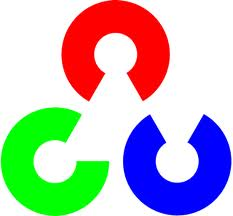
\includegraphics[width=0.6\textwidth]{Figures/OpenCVLogo.png}
      \end{figure}
    \end{column}
    \begin{column}{0.5\textwidth}
      OpenCV es una biblioteca libre de visión artificial, originalmente desarrollada por Intel.
      
      Programación en código  Python, C y C++
      
      Existen versiones para GNU/Linux, Mac OS X y Windows
    \end{column}
    \end{columns}
    \end{frame}

\begin{frame}\frametitle{OpenCV}
\begin{figure}[h!]
        \centering
        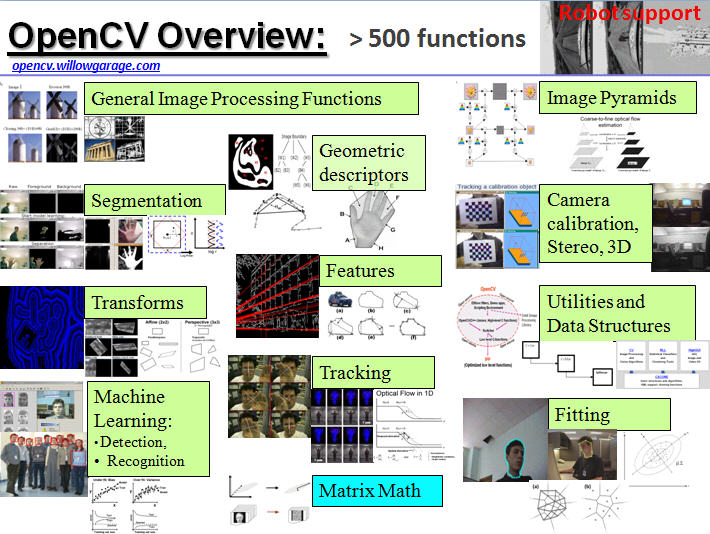
\includegraphics[width=0.75\textwidth]{Figures/OpenCVOverview.png}
\end{figure}
\end{frame}

\begin{frame}\frametitle{Funciones básicas}
  En Python, OpenCV está basado en la biblioteca Numpy por lo que muchas operaciones con imágenes corresponden a operaciones de Numpy sobre matrices.
  Algunas funciones que se usarán frecuentemente a lo largo del curso son:
  \begin{columns}
    \begin{column}{0.5\textwidth}
      \begin{itemize}
      \item \texttt{numpy.zeros}
      \item \texttt{enumpy.ones}
      \item \texttt{cv2.imread}
      \item \texttt{cv2.bitwise\_and}
      \item \texttt{cv2.bitwise\_or}
      \item \texttt{cv2.bitwise\_not}
      \item \texttt{cv2.bitwise\_xor}
      \end{itemize}
    \end{column}
    \begin{column}{0.5\textwidth}
      \begin{itemize}
      \item \texttt{cv2.inRange}
      \item \texttt{cv2.merge}
      \item \texttt{cv2.split}
      \item \texttt{cv2.imshow}
      \item \texttt{cv2.VideoCapture}
      \item \texttt{cv2.mean}
      \end{itemize}
    \end{column}
  \end{columns}
\end{frame}

\begin{frame}[containsverbatim]\frametitle{Ejercicio 1 - Lectura de imágenes y manejo de matrices}
  Escriba el siguiente código en un editor de texto:
  \lstinputlisting[language=Python]{Codes/Exercise01.py}
  Descargue la imagen \texttt{baboon.jpg} en la misma carpeta que el código. Abra una terminal y ejecute el código con el comando:
\begin{verbatim}
  python3 Exercise01.py
\end{verbatim}
  Modifique manualmente el tamaño de la imagen y modifique el código para que funcione con la imagen modificada. 
\end{frame}

\begin{frame}\frametitle{Operaciones lógicas}
  \begin{itemize}
  \item Las operaciones lógicas se usan generalmente para implementar \textit{máscaras}
  \item Puesto que son operaciones bit a bit, las imágenes a operar deben ser del mimo tamaño y tipo (mismo número de canales y mismo tipo de dato)
  \item Las máscaras suelen provenir de operaciones que dan como resultado imágenes binarias, como operaciones de comparación, umbralización o detección de bordes. 
  \end{itemize}
\end{frame}

\begin{frame}[containsverbatim]\frametitle{Ejercicio 2 - Operaciones lógicas bit a bit}
  Escriba el siguiente código en un editor de texto:
  \lstinputlisting[language=Python]{Codes/Exercise02.py}
  Ejecute el código y observe lo que hace cada operación.
\end{frame}

\begin{frame}[containsverbatim]\frametitle{Ejercicio 3 - Controles gráficos}
  \begin{itemize}
  \item OpenCV provee controles de interfaz gráfica de usuario que son útiles para la depuración de programas.
  \item Las barras de seguimiento (\textit{trackbars}) sirven para fijar valores en un intervalo y disparan una función \textit{callback} cuando hay un cambio en el valor.
  \item También provee \textit{callbacks} para el manejo de eventos del mouse (clicks derecho e izquierdo, movimiento del puntero, etc.)
  \end{itemize}
  Descargue el archivo \texttt{Exercise03.py}, ejecútelo y observe el comportamiento de la barra de seguimiento y de los clicks derecho e izquierdo. Consulte la documentación en línea y modifique el código para que se dibujen rectángulos con dimensiones dadas por dos clicks. 
\end{frame}

\begin{frame}\frametitle{Manejo de video}
  \begin{itemize}
  \item OpenCV provee la función \texttt{VideoCapture} para abrir fácilmente una cámara de video
  \item El video se entrega como una secuencia de imágenes por lo que un programa que maneje video debe contener un cilo \textit{while}
  \item La resolución más común es la de VGA de 640x480 aunque se pueden usar otras resoluciones dependiendo de las capacidades de cada cámara
  \item El número de cuadros por segundo (\textit{fps}) suele ser de 30, aunque puede ser de 60 o más, dependiendo de las capacidades de la cámara
  \item Si hay más de una cámara conectada, OpenCV las enumera con índices $i=0,1,2,3,\dots$ y se puede elegir qué cámara abrir usando dicho índice
  \item La misma funcion \texttt{VideoCapture} se puede usar para abrir videos en distintos formatos
  \end{itemize}
\end{frame}

\begin{frame}[containsverbatim]\frametitle{Ejercicio 4 - Manejo de vídeo}
  Escriba el siguiente código en un editor de texto:
  \lstinputlisting[language=Python]{Codes/Exercise04.py}
  El código anterior sólo abre una cámara y despliega la imagen en una ventana. Modifique el código para que realice lo siguiente:
  \begin{itemize}
  \item Cree una imagen en blanco y negro de dimensiones apropiadas similar a la del ejercicio 2
  \item Realice una o más operaciones lógicas entre el video y la imagen en blanco y negro
  \item Despliegue el resultado en una ventana
  \end{itemize}
\end{frame}
